\documentclass[11pt,a4j]{jsarticle}
\title{アナログ回路Ⅱ}
\author{1413176 三村幸祐}
\date{2016/11/09 \, 2016/11/16}
\usepackage{booktabs}
\usepackage[dvipdfmx,hiresbb]{graphicx}
%\pagestyle{empty}

\begin{document}
  
% \tableofcontents
% \newpage
  
 \section{目的}
 アナログ回路に我々が期待する機能とは、様々な演算機能を持っており、それらを回路に委託すれば答えが帰ってくることである。
 
  その一例として、現在までに私たちは線形信号処理のアナログ回路について学んできた。これにより和、差、乗算、周波数フィルタリング、微分積分などを回路上で表現することが可能となった。
  
  しかし、その他の非線形の演算を行う場合これらの知識では足りない。それを補うのが今回の実験の目的であり、リミッタ回路による出力のデジタル表現、ヒステリシスコンパレータによる可逆性の入出力循環変化、絶対値回路による閾値付近の性質変化による線形の折れ曲がり、などによって主に入出力特性が折れ線で表現される非線形信号処理について理解する。
  
  
 \section{レベルシフタ}
  \subsection{原理}
   
   \begin{figure}[htbp]
  \centering
  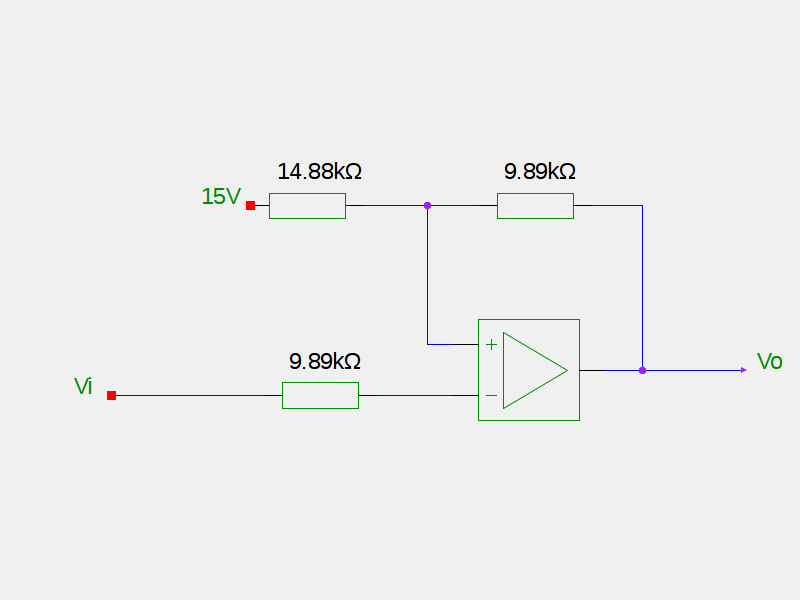
\includegraphics[width=8cm,clip]{levelshifter.png}
  \caption{レベルシフタの設計回路}
  \label{fig:levelshifter}
 \end{figure}%
   
  \subsection{測定手順}
   
   
  \subsection{結果と考察}
  レベルシフタの動作結果を図\ref{fig:1_0}に示した。この図を見ると、0~12Vの正の入力に対して、-10~10Vの一定の幅を持った正負の出力範囲が得られていることが分かる。したがってこれはレベルシフタとしての動作を反映していることを示し、さらに入力電圧に対して線形関数的に出力電圧が得られるため、以降実験の入力としてこの出力電圧を扱うに当たって、レベルシフタは非常に実験者からみても安定的で有効な回路である、ということが分かった。
  
   \begin{figure}[htbp]
  \centering
  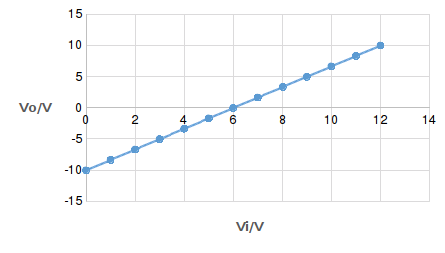
\includegraphics[width=8cm,clip]{1_0.png}
  \caption{レベルシフタの測定測定}
  \label{fig:1_0}
 \end{figure}%
   
 \section{リミッタ}
  \subsection{オペアンプを用いないリミッタの入出力特性}
   \subsubsection{原理}
    
    \begin{figure}[htbp]
  \centering
  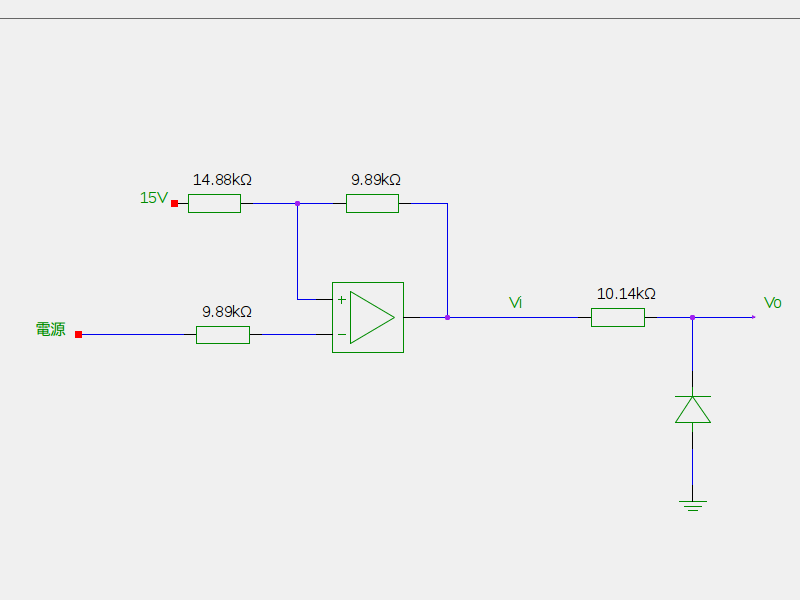
\includegraphics[width=8cm,clip]{noamp_tokusei.png}
  \caption{オペアンプを用いないリミッタの測定回路}
  \label{fig:noamp_tokusei}
 \end{figure}%
    
   \subsubsection{測定手順}
    
    
   \subsubsection{結果と考察}
    図\ref{fig:1_1_noamp_PS}にオペアンプを用いないリミッタの入出力特性を示す。
    この図を見ると、入力電圧が正の時は傾きが1の線形特性、入力電圧が負の時は0に近い一定の負の出力が得られることが分かる。リミッタ回路の特性上、入力が負の場合には回路上のダイオードに正のバイアスが、入力が正の場合にはダイオードに負のバイアスがかかる。つまりリミッタ回路の入出力特性は以下のようにまとめることができる。
    \begin{itemize}
    \item 入力電圧$V_i < 0$Vの時、出力電圧$V_o$は0V
    \item 入力電圧$V_i > 0$Vの時、出力電圧$V_o$=$V_i$
    \end{itemize}
    
    
    \begin{figure}[htbp]
  \centering
  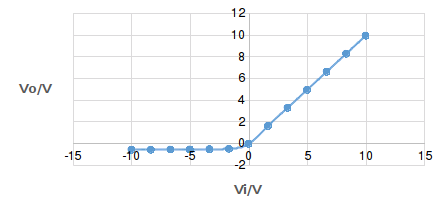
\includegraphics[width=8cm,clip]{1_1_noamp_PS.png}
  \caption{オペアンプを用いないリミッタの入出力特性}
  \label{fig:1_1_noamp_PS}
 \end{figure}%
    
    これでリミッタ回路の入出力特性を確認することができたわけだが、ダイオードをスイッチとして使用した例である。この図からは入力電圧が微小な負の値をもつ所から出力電圧が立ち上がり始めていることも確認できるため、ダイオードの立ち上がり電圧もデータに現れていることもわかる。
    
  \subsection{オペアンプを用いないリミッタの入出力波形観測}
   \subsubsection{原理}
    
    \begin{figure}[htbp]
  \centering
  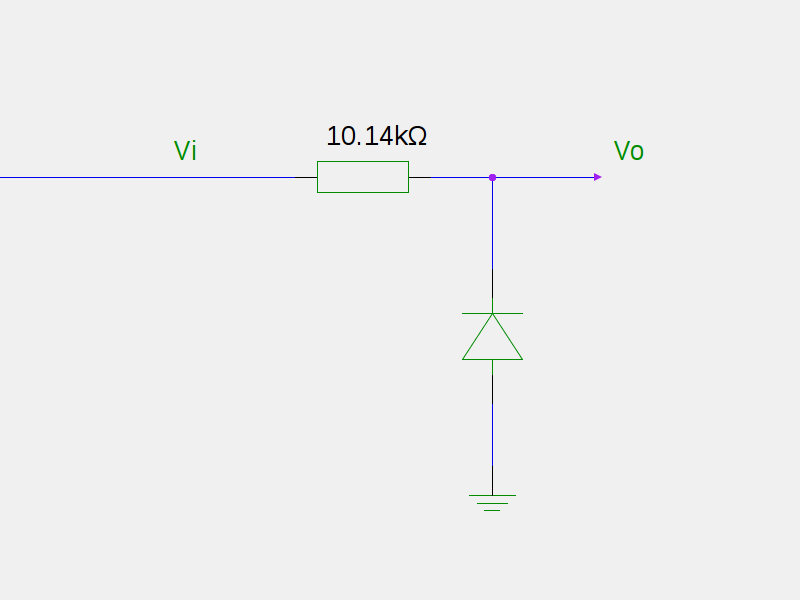
\includegraphics[width=8cm,clip]{noamp_wave.png}
  \caption{オペアンプを用いないリミッタの波形観測回路}
  \label{fig:noamp_wave}
 \end{figure}%
    
   \subsubsection{測定手順}
    
    
   \subsubsection{結果と考察}
    
    オペアンプを用いないリミッタの入出力波形を、正弦波、入力周波数、電圧によって測定した3つのサンプルデータをそれぞれ図\ref{fig:noamp_f1V2}、図\ref{fig:noamp_sankaku}、図\ref{fig:noamp_f100V4}に示す。
    
    
    \begin{figure}[htbp]
  \centering
  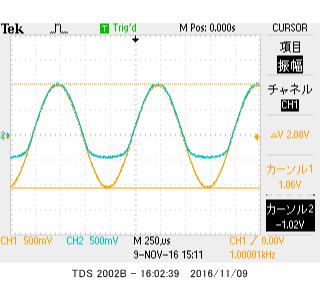
\includegraphics[width=8cm,clip]{1_1_noampFG_f1V2_ViVo.png}
  \caption{オペアンプを用いないリミッタの入出力波形(正弦波,入力周波数1kHz,電圧2Vpp)}
  \label{fig:noamp_f1V2}
 \end{figure}%
 
 \begin{figure}[htbp]
  \centering
  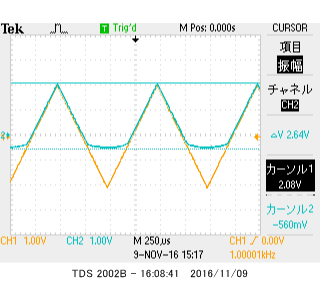
\includegraphics[width=8cm,clip]{1_1_noampFG_f1V4sankaku_ViVo.png}
  \caption{オペアンプを用いないリミッタの入出力波形(三角波,入力周波数1kHz,電圧4Vpp)}
  \label{fig:noamp_sankaku}
 \end{figure}%
 
 \begin{figure}[htbp]
  \centering
  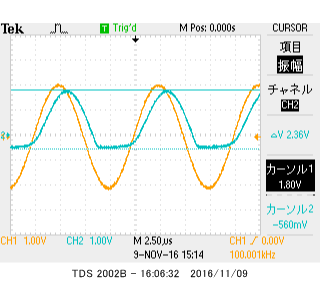
\includegraphics[width=8cm,clip]{1_1_noampFG_f100V4_ViVo.png}
  \caption{オペアンプを用いないリミッタの入出力波形(正弦波,入力周波数100kHz,電圧4Vpp)}
  \label{fig:noamp_f100V4}
 \end{figure}%
    
    入力周波数が1kHzの2つのデータを見てみると、入力が正の領域で入出力が1対1の関係になっている。負の方向に少し出力が浸透しているものダイオードの立ち上がり電圧による影響であろう。
    一方、入力周波数が100kHzのデータは振幅だけなら大きな変化はないものの、時間的な遅延が生じていることが確認できる。これはダイオードの含有する静電容量によるものだと考えられ、周波数が大きくなるとさらに大きな影響を及ぼすものだと予測できる。
    
    したがってここから、リミッタ回路は直流利用では問題なく利用できるが、交流として利用する際には、使用する周波数帯には気をつけなければならないということが分かった。
    
    
  \subsection{オペアンプを用いたリミッタの入出力特性}
   \subsubsection{原理}
    
    \begin{figure}[htbp]
  \centering
  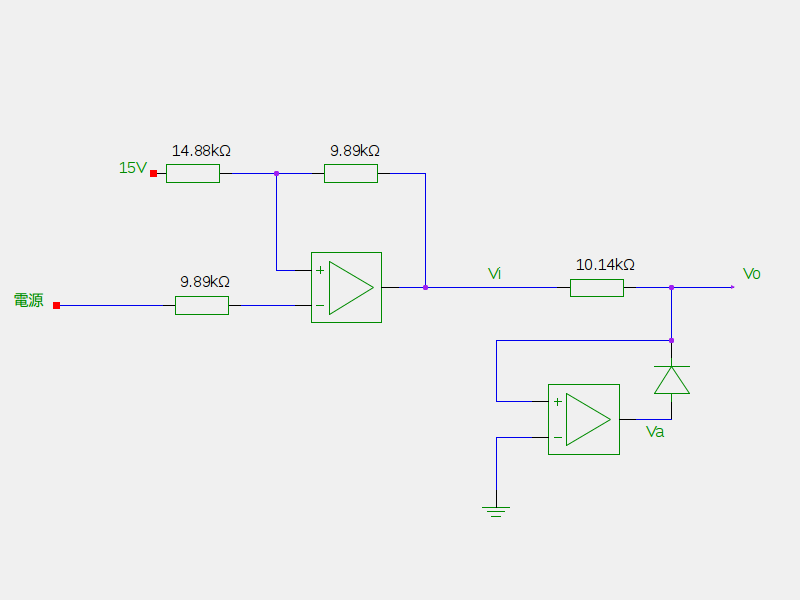
\includegraphics[width=8cm,clip]{amp_tokusei.png}
  \caption{オペアンプを用いたリミッタの測定回路}
  \label{fig:amp_tokusei}
 \end{figure}%
    
   \subsubsection{測定手順}
    
    
   \subsubsection{結果と考察}
    次の図\ref{fig:1_1_amp_PS_ViVo}、図\ref{fig:1_1_amp_PS_ViVa}にそれぞれ入力電圧に対するリミッタの出力、そしてオペアンプの出力電圧特性を示した。
    
    まず図\ref{fig:1_1_amp_PS_ViVo}をみてみる。このデータは定性的には先述のオペアンプを用いない場合の入出力特性と同様に見える。しかし今回の場合はマイナス側への出力電圧の浸透がなく、さらに立ち上がり部分の0に近づいている。
    
    さらに図\ref{fig:1_1_amp_PS_ViVa}を見ると、入力の0Vを境に離散的にオペアンプの出力は0Vから-14Vまで変わっている。このオペアンプの性質によって、オペアンプありのオペアンプなしとの違いは、
    \begin{itemize}
    \item リミット電圧のスイッチとしてのon,offへの切り替え性能の向上
    \item スイッチoff時の電圧漏れだしの防止
    \end{itemize}
    などが主にあげられる。
    
    \begin{figure}[htbp]
  \centering
  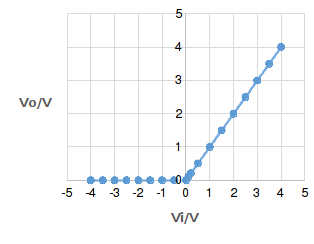
\includegraphics[width=8cm,clip]{1_1_amp_PS_ViVo.png}
  \caption{オペアンプを用いたリミッタの入出力特性}
  \label{fig:1_1_amp_PS_ViVo}
 \end{figure}%
   
   \begin{figure}[htbp]
  \centering
  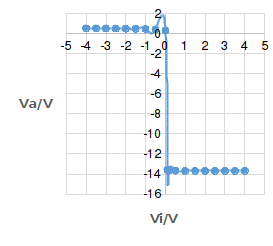
\includegraphics[width=8cm,clip]{1_1_amp_PS_ViVa.png}
  \caption{リミッタの入力電圧とオペアンプの出力電圧の特性}
  \label{fig:1_1_amp_PS_ViVa}
 \end{figure}%
    
    
  \subsection{オペアンプを用いたリミッタの入出力波形観測}
   \subsubsection{原理}
    
    \begin{figure}[htbp]
  \centering
  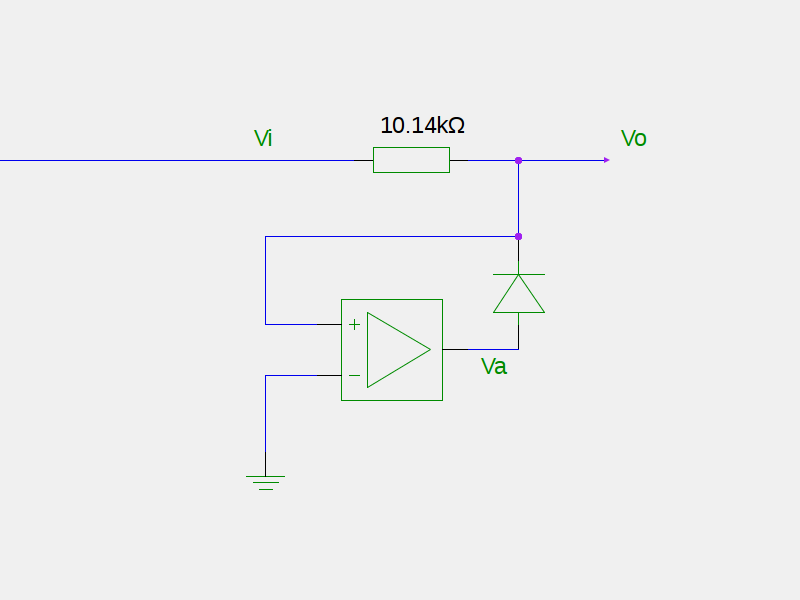
\includegraphics[width=8cm,clip]{amp_wave.png}
  \caption{オペアンプを用いたリミッタの波形観測回路}
  \label{fig:amp_wave}
 \end{figure}%
    
   \subsubsection{測定手順}
    
    
   \subsubsection{結果と考察}
    図\ref{fig:ampFGf1v2vivo},\ref{fig:ampFGf1v2viva}に正弦波で周波数1kHzの入力に対するデータを、図\ref{fig:ampFGf1v4vivo},\ref{fig:ampFGf1v4viva}に三角波で周波数1kHzの入力に対するデータを、そして最後の図\ref{fig:ampFGf100v4}に正弦波で周波数1kHzの入力に対するデータを示す。
    
    ここでも上述の入出力特性に関する特性と同様に、周波数が1kHzで低い状態ではその挙動はオペアンプなしと変わらない。
    
    \begin{figure}[htbp]
  \centering
  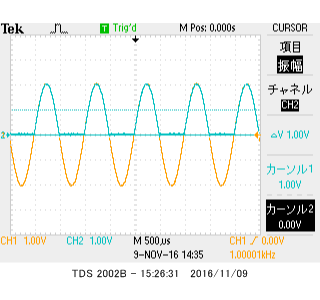
\includegraphics[width=8cm,clip]{1_1_ampFG_f1V2_ViVo.png}
  \caption{オペアンプを用いたリミッタの入出力波形(正弦波,入力周波数1kHz,電圧2Vpp)}
  \label{fig:ampFGf1v2vivo}
 \end{figure}%
 
 \begin{figure}[htbp]
  \centering
  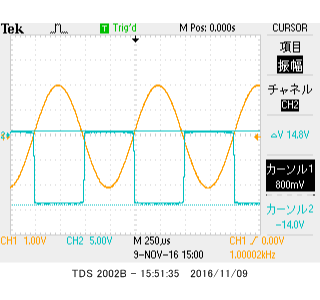
\includegraphics[width=8cm,clip]{1_1_ampFG_f1V2_ViVa.png}
  \caption{リミッタの入力電圧とオペアンプの出力電圧(正弦波,入力周波数1kHz,電圧2Vpp)}
  \label{fig:ampFGf1v2viva}
 \end{figure}%
 
 \begin{figure}[htbp]
  \centering
  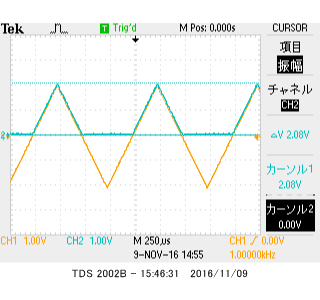
\includegraphics[width=8cm,clip]{1_1_ampFG_f1V4sankaku_ViVo.png}
  \caption{オペアンプを用いたリミッタの入出力波形(三角波,入力周波数1kHz,電圧4Vpp)}
  \label{fig:ampFGf1v4vivo}
 \end{figure}%
 
 \begin{figure}[htbp]
  \centering
  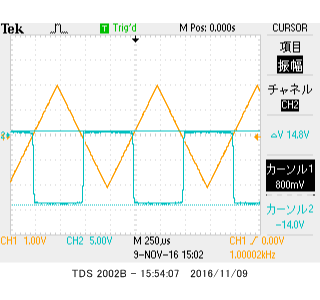
\includegraphics[width=8cm,clip]{1_1_ampFG_f1V4sankaku_ViVa.png}
  \caption{リミッタの入力電圧とオペアンプの出力電圧(三角波,入力周波数1kHz,電圧4Vpp)}
  \label{fig:ampFGf1v4viva}
 \end{figure}%
 
 \begin{figure}[htbp]
  \centering
  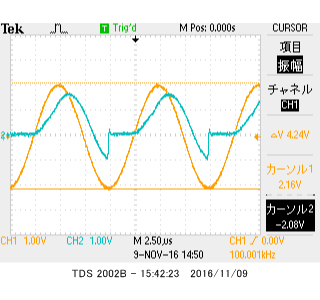
\includegraphics[width=8cm,clip]{1_1_ampFG_f100V4_ViVo.png}
  \caption{オペアンプを用いたリミッタの入出力波形(正弦波,入力周波数100kHz,電圧4Vpp)}
  \label{fig:ampFGf100v4}
 \end{figure}%
  
  
    
  
 \section{ヒステリシスコンパレータ回路}
  \subsection{ヒステリシスコンパレータの入出力特性}
   \subsubsection{原理}
    
    \begin{figure}[htbp]
  \centering
  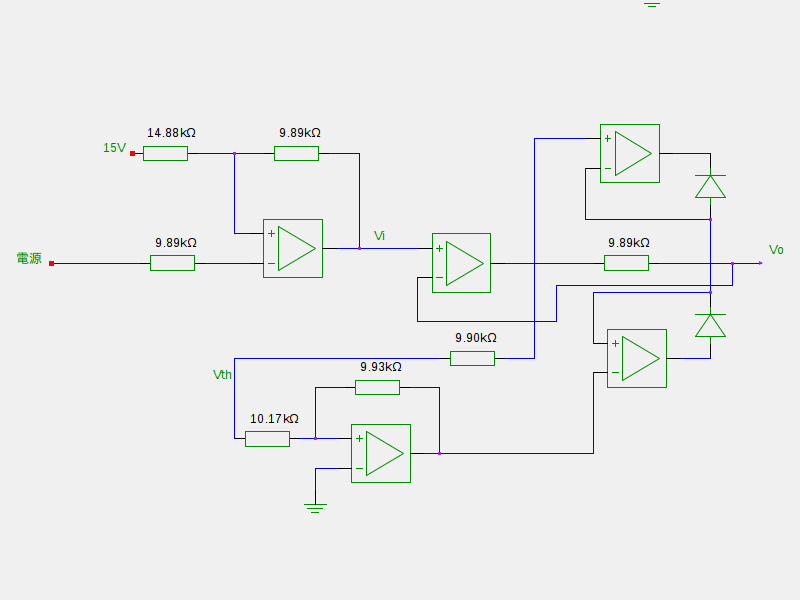
\includegraphics[width=8cm,clip]{histeri_tokusei.png}
  \caption{ヒステリシスコンパレータの測定回路}
  \label{fig:histeri_tokusei}
 \end{figure}%
    
   \subsubsection{測定手順}
    
    
   \subsubsection{結果と考察}
    PS出力電圧$V_{th}$を2V,1Vとして測定したヒステリシスのデータをそれぞれ図\ref{fig:1_2_histeri_Vth2},図\ref{fig:1_2_histeri_Vth1}に示す。
    
    \begin{figure}[htbp]
  \centering
  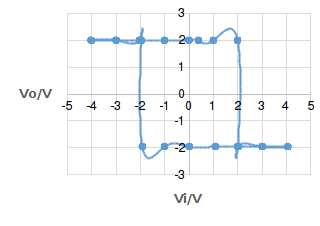
\includegraphics[width=8cm,clip]{1_2_histeri_Vth2.png}
  \caption{PS出力電圧$V_{th}$=2Vの時のヒステリシスコンパレータの入出力特性}
  \label{fig:1_2_histeri_Vth2}
 \end{figure}%
    
 \begin{figure}[htbp]
  \centering
  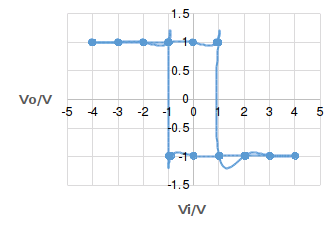
\includegraphics[width=8cm,clip]{1_2_histeri_Vth1.png}
  \caption{PS出力電圧$V_{th}$=1Vの時のヒステリシスコンパレータの入出力特性}
  \label{fig:1_2_histeri_Vth1}
 \end{figure}%
    
    
    
  \subsection{ヒステリシスコンパレータの入出力波形観測}
   \subsubsection{原理}
    
    \begin{figure}[htbp]
  \centering
  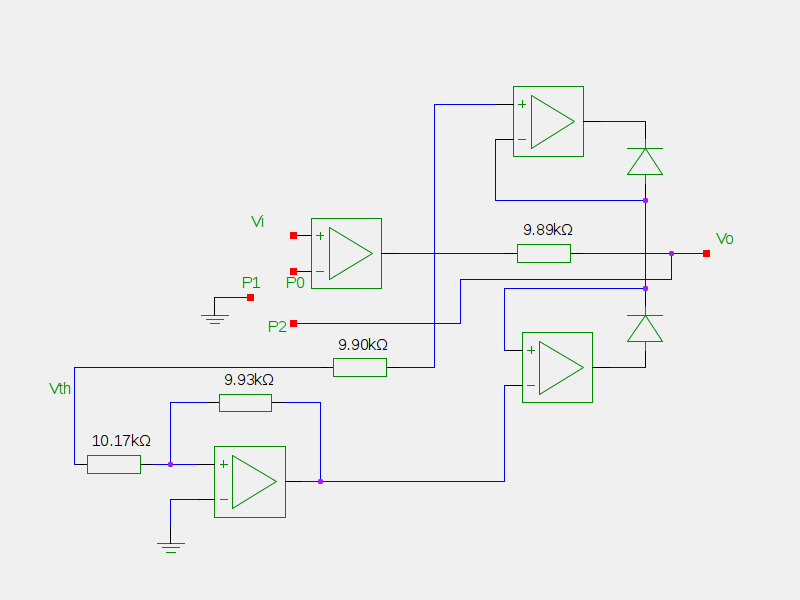
\includegraphics[width=8cm,clip]{histeri_wave.png}
  \caption{ヒステリシスコンパレータの波形観測回路}
  \label{fig:histeri_wave}
 \end{figure}%
    
   \subsubsection{測定手順}
    
    
   \subsubsection{結果と考察}
    
    
 \section{絶対値回路}
  \subsection{絶対値回路の入出力特性}
   \subsubsection{原理}
    
    \begin{figure}[htbp]
  \centering
  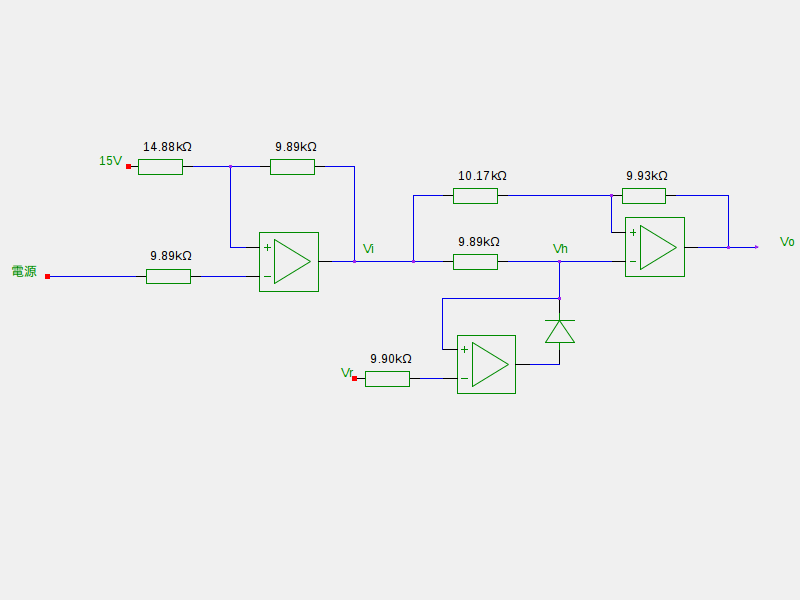
\includegraphics[width=8cm,clip]{abs_tokusei.png}
  \caption{絶対値回路の測定回路}
  \label{fig:abs_tokusei}
 \end{figure}%
    
   \subsubsection{測定手順}
    
    
   \subsubsection{結果と考察}
    
    \begin{figure}[htbp]
  \centering
  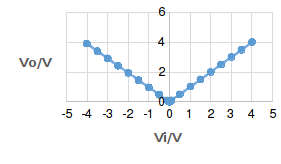
\includegraphics[width=8cm,clip]{2_Vr0.png}
  \caption{基準電圧$V_r$=0Vの時の絶対値回路の入出力特性}
  \label{fig:2_Vr0}
 \end{figure}%
    
    \begin{figure}[htbp]
  \centering
  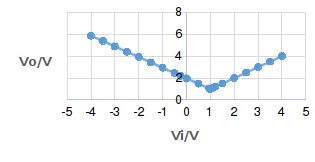
\includegraphics[width=8cm,clip]{2_Vr1.png}
  \caption{基準電圧$V_r$=1Vの時の絶対値回路の入出力特性}
  \label{fig:2_Vr1}
 \end{figure}%
    
    
    
  \subsection{絶対値回路の入出力波形測定}
   \subsubsection{原理}
    
    \begin{figure}[htbp]
  \centering
  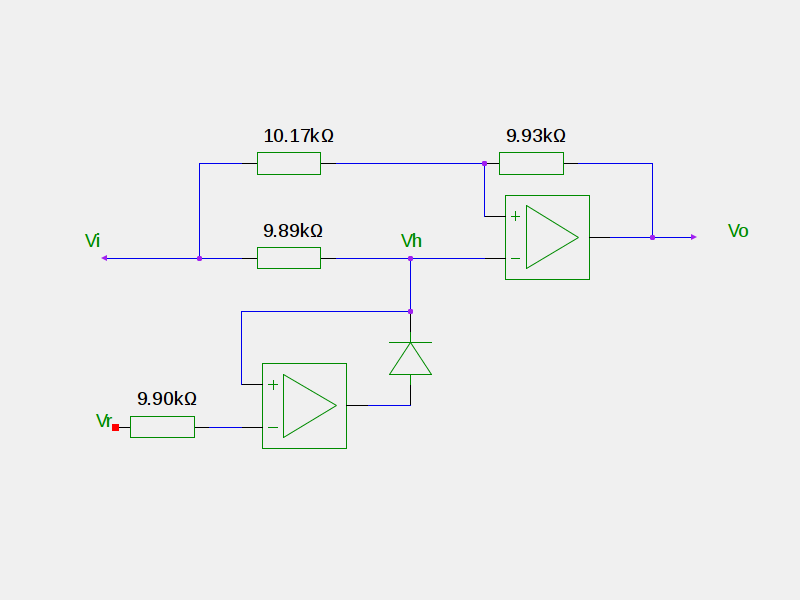
\includegraphics[width=8cm,clip]{abs_wave.png}
  \caption{絶対値回路の波形観測回路}
  \label{fig:abs_wave}
 \end{figure}%
    
   \subsubsection{測定手順}
    
    
   \subsubsection{結果と考察}
    
    \begin{figure}[htbp]
  \centering
  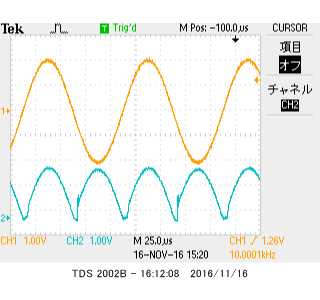
\includegraphics[width=8cm,clip]{2_abs_Vr0_f10V4sin_ViVo.png}
  \caption{基準電圧なしの絶対値回路の波形(f=10kHz,Vpp=4V,正弦波)}
  \label{fig:2_Vr0_sin}
 \end{figure}%
    
    
    \begin{figure}[htbp]
  \centering
  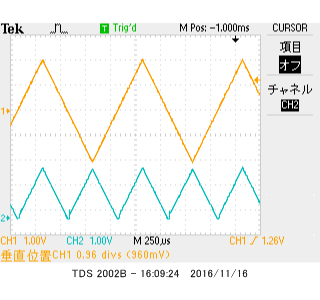
\includegraphics[width=8cm,clip]{2_abs_Vr0_f1V4sankaku_ViVo.png}
  \caption{基準電圧なしの絶対値回路の波形(f=1kHz,Vpp=4V,三角波)}
  \label{fig:2_Vr0_sankaku}
 \end{figure}%
  
  \begin{figure}[htbp]
  \centering
  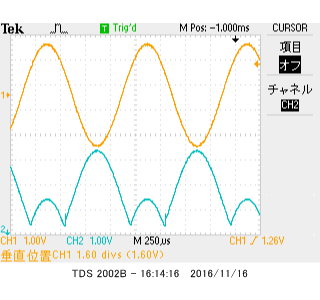
\includegraphics[width=8cm,clip]{2_abs_Vr1_f1V2sin_ViVo.png}
  \caption{基準電圧1Vの絶対値回路の波形(f=1kHz,Vpp=2V)}
  \label{fig:2_Vr1_2}
 \end{figure}%
  
  
  \begin{figure}[htbp]
  \centering
  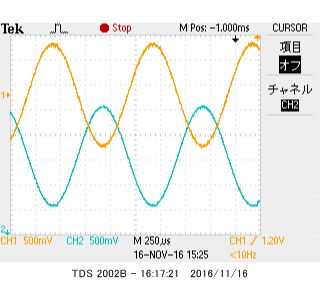
\includegraphics[width=8cm,clip]{2_abs_Vr1_f1V4sin_ViVo.png}
  \caption{基準電圧1Vの絶対値回路の波形(f=1kHz,Vpp=4V)}
  \label{fig:2_Vr1_4}
 \end{figure}%
  
 \section{レポート課題} 
  
  
 \section{参考文献}
  
  
  
\end{document}